% This is samplepaper.tex, a sample chapter demonstrating the
% LLNCS macro package for Springer Computer Science proceedings;
% Version 2.20 of 2017/10/04
%
\documentclass[runningheads]{llncs}
%
\usepackage{graphicx}
% Used for displaying a sample figure. If possible, figure files should
% be included in EPS format.
%
% If you use the hyperref package, please uncomment the following line
% to display URLs in blue roman font according to Springer's eBook style:
% \renewcommand\UrlFont{\color{blue}\rmfamily}

\begin{document}
%
\title{Literary Studies Meet Corpus Linguistics: Estonian Pilot Project of Private Letters in KORP\thanks{Supported by organization x.}}
%
\titlerunning{Private Letters in KORP}
% If the paper title is too long for the running head, you can set
% an abbreviated paper title here
%
\author{Marin Laak\inst{1} \and Kaarel Veskis\inst{1} \and\\
Olga Gerassimenko\inst{2} \and Neeme Kahusk\inst{2} \and
Kadri Vider\inst{2}}
%
\authorrunning{M. Laak et al.}
% First names are abbreviated in the running head.
% If there are more than two authors, 'et al.' is used.
%
\institute{Estonian Literary Museum\\
  Vanemuise 42, 51003 Tartu, Estonia\\
\email{\{marin.laak,kaarel.veskis\}@kirmus.ee}\and
Institute of Computer Science, University of Tartu,\\
J. Liivi 2, 50409 Tartu, Estonia
\email{\{olga.gerassimenko,neeme.kahusk,kadri.vider\}@ut.ee}
}
%
\maketitle              % typeset the header of the contribution
%
\begin{abstract}
  Digitisation of cultural heritage in Estonia has been in progress during recent years, and we will see expansive mass digitalisation of printed books and handwritten dokuments in the very near future.
  
  This situation and potential actualises the questions of the usage of the literary heritage. In our paper, we consider the benefits for the digital literary research that arise from representing a literary text collection as a linguistically annotated language resource. We discuss the pilot project of creating a DH corpus based on private letters between two avangardist writers  Johannes Semper and Johannes Barbarus during the first Estonian Republic in the beginning of the 20. century.
  
The advantages and possibilities of corpus search system KORP that we have chosen for representing and searching literary heritage DH corpora as a language resource are described. Challenges that application of Natural Language Processing and Text and Data Mining imposes on the preparation and representation of the texts are discussed along with the benefits for the research. 


\keywords{literary studies \and private letters \and digital heritage collections \and corpus linguistics \and data mining \and natural language processing}

\end{abstract}
%
%
%
\section{Introduction}

The application of Language Technology (LT) and Text and Data Mining (TDM) methods and tools is gradually increasing and becoming more relevant in Estonia. Similarly to the Nordic and Baltic countries, Estonia can expect an explosive growth of digital heritage and text resources: preparations for massive digitisation of cultural heritage started in 2019 as national programme. The creation of these new digital resources will be the priority for all Estonian leading memory institutions and the scope of this huge project includes all different types of cultural heritage (printed books, archival documents, photo and film heritage, ethnographic and fine art objects) [5, 9] Digitized resources will be made accessible on the Internet as open data, but it is still an open question how and for what purpose can such digital resources be used [4]. 

What are the new challenges and the new knowledge offered by using the applications of Linguistic Analysis tools in analysing the digital literary heritage? Our interdisciplinary project “Literary Studies Meet Corpus Linguistics” concentrates on using cultural heritage, especially literary history sources in research with the help of the LT\&TDM methods. The primary question is how to bridge the gap between the research possibilities offered by the contemporary LT\&TDM and the ever increasing resources of texts and other digital data, produced by memory institutions. This has proved to be a complicated task and international practice has shown that literary scholars are slower to embrace new practices than linguists for whom corpus-based research is already a professional standard. In general, literary scholars are used to working with texts with traditional methods, analysing them as undivided poetical and semantic entities [9]. Digitizing of texts often preserves them as undivided and unannotated entities with occasionally added metadata - as a result, the digitized materials are human-readable rather than machine-readable.

LT\&TDM methods require treating literary works or texts as data, which can be analysed and processed with computer programmes. To research for statistics and trends in the data, a literary scholar needs either to do a close reading of literary texts as huge data amounts, or to develop new professional skills in data analysis methods. This imposes rethinking the approach to empirical object in literary studies in general and posing new and different research questions. The possibility to compare text strategies, rhetorical and stylistic patterns in literary, religious and political text corpora might give us new insights into intertwining ideology, rhetoric and identity presentations. One of the important trends of automated textual analysis in DH is Sentiment Analysis which, for instance, allows to measure emotion in parliamentary debates [6].


\section{Private letters as a literary source}

The empirical base of our pilot project of private letters in KORP is based on the archival ego-documents. This is a rare collection of handwritten private letters: the correspondence between two Estonian writers Johannes Semper (1892–1970) and Johannes Barbarus (1890–1946). The authors were well-known avant-garde writers in Estonian literature, best friends and school classmates. They shared the same intellectual attitudes, views, and values. For example, they were Francophiles and during several decades they both mediated and translated French literature into Estonian. 

During the years covered by the correspondence, in 1911-1939, Barbarus published the total of 17 collections of poetry, and Semper published four collections of poetry and four books of short stories and novels. The letters were written mainly in different places in Estonia, and also during travels: they both travelled extensively in Europe (and other parts of the world) and in their letters they described to each other the sights they saw as well as the literary events at home. They also wrote about their work, everyday life, health and prescriptions, hobbies (hunting, swimming, skating, etc.), and guests. 

The temporal and contextual frames of this correspondence is the period in Europe between two World Wars and, according to French philosopher Pierre Bourdieu, the creation of  the Estonian ‘cultural field’ in the Estonian Republic in years 1918-1940. As such, the correspondence offers semantically rich and multidimensional content for literary scholars.  

Generally, we are inspired by the question how this kind of sources (private letters, correspondences, manuscripts, etc.) in different kinds of computer-readable formats (pdf, docx, txt etc.) can be used for creating new knowledge in the interdisciplinary field of literary studies, including biographics and life writing studies [7]. 

The private correspondence of two Estonian writers during 28 years as an empirical material is extremely rich in the themes and possibilities to pose the traditional as well as the new research questions, e.g the factors of subjectivity and emotionality, verbal and poetic creativeness of the both authors.  

The original letters are held at different archives: the letters of Barbarus to Semper are at the Estonian Cultural History Archives of the Estonian Literary Museum and the letters of Semper to Barbarus are at the Estonian National Archives due to the unique literary and historical value of this correspondence. Why? Their correspondence consists of 670 letters with, all in all, more than 1,100 pages and more than 310 890 tokens (249 970 words). 


\section{KORP as a tool for corpus linguistics}

KORP is a corpus query analysis system that allows to find concordances and build various statistics from differently annotated corpora using text metadata (author, year of publishing, text type etc) and linguistic annotation (splitting into sentences and words, punctuation, morphology, syntax and semantics). Technically, KORP is a frontend tool that uses much of IMS Open Corpus Workbench as backend. It was created and maintained at Swedish Language Bank Språkbanken [1] and is being developed and customised by language technology networks in several countries: Sweden, Finland, Norway, Estonia, Denmark, Island and Italy (internal use in the University of Florence).  

Estonian KORP is hosted by the Centre of Estonian Language Resources. The Estonian data available for search in KORP currently consists of more than 850 million tokens. As Estonian is a highly inflective language with a rich morphology and free word order, almost all texts are automatically annotated and disambiguated on the morphological level to enable form- and baseform-based search.


As a pilot project for the needs of literary studies in addition to the corpora designed for linguistic research, we have added Correspondence Corpus of private letters (Semper and Barbarus, 1911-1940). The original handwritten manuscripts where already transformed to typewritten and then to electronic format; they had to be further transformed to a computer-readable text files by manually adding metadata and automatically analyzing and disambiguating morphological categories. 

KORP was chosen because of its open source value, search flexibility and easiness, graphical overview of search results in subcorpora, easy switching between concordances and broader context (as well as between statistics and concordances), broad possibilities to group search statistics and automatically created relative statistics (occurrences per million tokens).  The search results and statistics from the KORP are exportable to Comma Separated Values (CSV) format; we plan to extend the export to the Excel (XLS) and HTML formats (already used in Finnish KORP),  integrate a single sign-on access for corpora with restricted usage, introduce links to audio and video data, links to lexicons and automatic annotation of corpora, the features already implemented in KORP of the other countries (Finland, Sweden, Norway). Text fragments cited in KORP are limited to a sentence or a passage, so that KORP does not infringe copyrights,; metadata cited in the query results allow exact pinpointing of the source of the sentence, and there is a possibility to pint


\section{Challenges for annotation in manuscript corpus}


\subsection{A Subsection Sample}
Please note that the first paragraph of a section or subsection is
not indented. The first paragraph that follows a table, figure,
equation etc. does not need an indent, either.

Subsequent paragraphs, however, are indented.

\subsubsection{Sample Heading (Third Level)} Only two levels of
headings should be numbered. Lower level headings remain unnumbered;
they are formatted as run-in headings.

\paragraph{Sample Heading (Fourth Level)}
The contribution should contain no more than four levels of
headings. Table~\ref{tab1} gives a summary of all heading levels.

\begin{table}
\caption{Table captions should be placed above the
tables.}\label{tab1}
\begin{tabular}{|l|l|l|}
\hline
Heading level &  Example & Font size and style\\
\hline
Title (centered) &  {\Large\bfseries Lecture Notes} & 14 point, bold\\
1st-level heading &  {\large\bfseries 1 Introduction} & 12 point, bold\\
2nd-level heading & {\bfseries 2.1 Printing Area} & 10 point, bold\\
3rd-level heading & {\bfseries Run-in Heading in Bold.} Text follows & 10 point, bold\\
4th-level heading & {\itshape Lowest Level Heading.} Text follows & 10 point, italic\\
\hline
\end{tabular}
\end{table}


\noindent Displayed equations are centered and set on a separate
line.
\begin{equation}
x + y = z
\end{equation}
Please try to avoid rasterized images for line-art diagrams and
schemas. Whenever possible, use vector graphics instead (see
Fig.~\ref{fig1}).

\begin{figure}
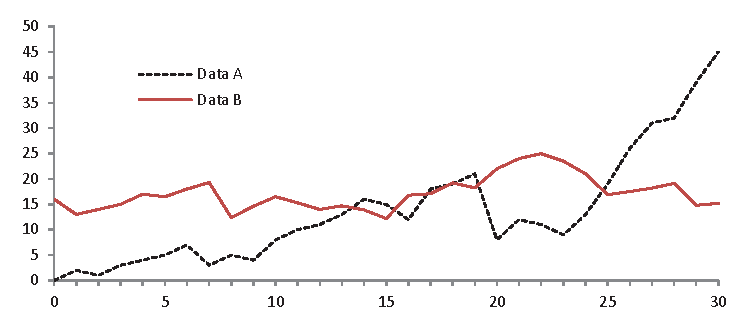
\includegraphics[width=\textwidth]{fig1.eps}
\caption{A figure caption is always placed below the illustration.
Please note that short captions are centered, while long ones are
justified by the macro package automatically.} \label{fig1}
\end{figure}

\begin{theorem}
This is a sample theorem. The run-in heading is set in bold, while
the following text appears in italics. Definitions, lemmas,
propositions, and corollaries are styled the same way.
\end{theorem}
%
% the environments 'definition', 'lemma', 'proposition', 'corollary',
% 'remark', and 'example' are defined in the LLNCS documentclass as well.
%
\begin{proof}
Proofs, examples, and remarks have the initial word in italics,
while the following text appears in normal font.
\end{proof}
For citations of references, we prefer the use of square brackets
and consecutive numbers. Citations using labels or the author/year
convention are also acceptable. The following bibliography provides
a sample reference list with entries for journal
articles~\cite{ref_article1}, an LNCS chapter~\cite{ref_lncs1}, a
book~\cite{ref_book1}, proceedings without editors~\cite{ref_proc1},
and a homepage~\cite{ref_url1}. Multiple citations are grouped
\cite{ref_article1,ref_lncs1,ref_book1},
\cite{ref_article1,ref_book1,ref_proc1,ref_url1}.
%
% ---- Bibliography ----
%
% BibTeX users should specify bibliography style 'splncs04'.
% References will then be sorted and formatted in the correct style.
%
% \bibliographystyle{splncs04}
% \bibliography{mybibliography}
%
\begin{thebibliography}{8}
\bibitem{ref_article1}
Author, F.: Article title. Journal \textbf{2}(5), 99--110 (2016)

\bibitem{ref_lncs1}
Author, F., Author, S.: Title of a proceedings paper. In: Editor,
F., Editor, S. (eds.) CONFERENCE 2016, LNCS, vol. 9999, pp. 1--13.
Springer, Heidelberg (2016). \doi{10.10007/1234567890}

\bibitem{ref_book1}
Author, F., Author, S., Author, T.: Book title. 2nd edn. Publisher,
Location (1999)

\bibitem{ref_proc1}
Author, A.-B.: Contribution title. In: 9th International Proceedings
on Proceedings, pp. 1--2. Publisher, Location (2010)

\bibitem{ref_url1}
LNCS Homepage, \url{http://www.springer.com/lncs}. Last accessed 4
Oct 2017
\end{thebibliography}
\end{document}
